\begin{figure}[htbp]
\vspace{-0.5 cm}
\setlength{\abovecaptionskip}{0.2 cm}   
\setlength{\belowcaptionskip}{-0.56 cm} 
    \centering
    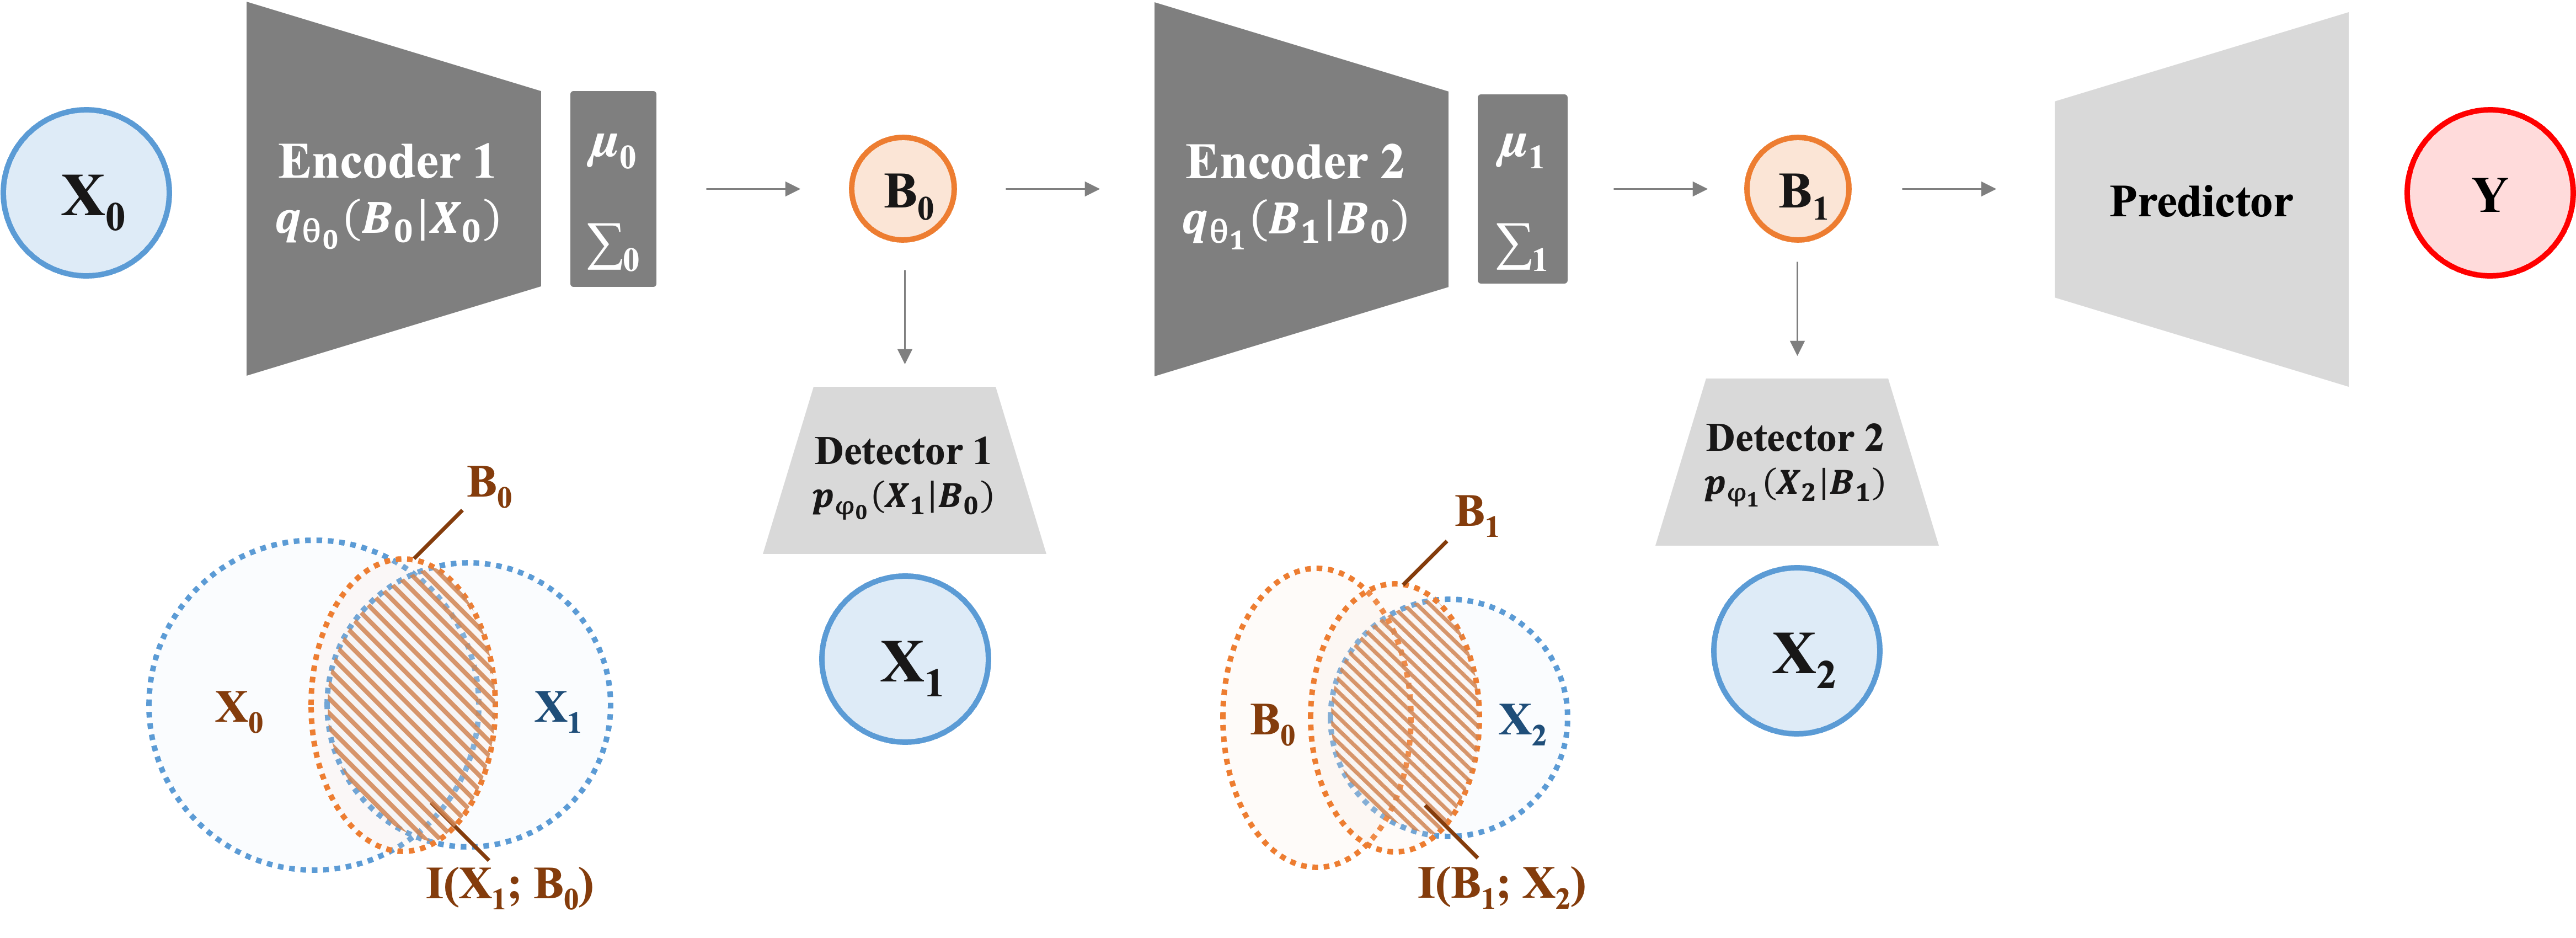
\includegraphics[width=.96\linewidth]{Figures/Model.png}
    \caption{\textbf{An illustration of the proposed model architecture.} In each encoder, we have two MLP layers: the initial layer extracts the feature vectors from input states, while the second layer generates parameters for the latent Gaussian distribution. The Venn diagrams illustrate the information constraint from  the optimization problem (\ref{eqn:optimProb}).}
    \label{fig:model}
\end{figure}